\documentclass[11pt,a4paper]{article}
\usepackage[T1]{fontenc}
\usepackage{lmodern,microtype,amsmath,amssymb,amsthm,mathtools,booktabs,tabularx,array}
\usepackage[top=23mm,bottom=23mm,left=26mm,right=26mm,headheight=14pt]{geometry}
\usepackage[svgnames]{xcolor}
\usepackage{fancyhdr,enumitem,pgfplots}
\pgfplotsset{compat=1.17}
\usepackage{fvextra}
\usepackage{hyperref}
\definecolor{ink}{HTML}{16343A}
\definecolor{accent}{HTML}{14605D}
\hypersetup{colorlinks=true,linkcolor=accent,urlcolor=accent,citecolor=accent,
pdftitle={Higher differences of exponential remainders},pdfsubject={Gautschi's conjecture, Sitnik's order questions and Brezinski's tail question}}
\pagestyle{fancy}\fancyhf{}
\fancyhead[L]{\small\color{ink}Higher differences of exponential remainders}
\fancyhead[R]{\small\color{ink}Research manuscript}
\fancyfoot[C]{\small\thepage}
\newtheorem{theorem}{Theorem}[section]
\newtheorem{lemma}[theorem]{Lemma}
\newtheorem{corollary}[theorem]{Corollary}
\newtheorem{proposition}[theorem]{Proposition}
\setlength{\emergencystretch}{2em}
\setlist{nosep}
\raggedbottom
\begin{document}
\thispagestyle{plain}
\begin{center}
{\small\sffamily\color{accent} SPECIAL FUNCTIONS AND FINITE DIFFERENCES}\par\vspace{8pt}
{\LARGE\bfseries\color{ink}Higher differences of exponential remainders}\par\vspace{5pt}
{\large Gautschi's conjecture, Sitnik's order questions and Brezinski's tail question}\par\vspace{7pt}
{\small Keio and Shaitetsu \quad $\cdot$ \quad 21 November 2026}
\end{center}
\begin{abstract}
We prove Gautschi's 1982 conjecture that the mean-value point $\theta_n(x)$ of the exponential remainder satisfies $\Delta^3\theta_n(x)<0$ for every $n\ge0$ and real $x\ne0$. The proof for positive arguments realizes a logarithmic derivative as the third central moment of a variable clipped at zero. A Gaussian transition shows that every order $k\ge4$ takes both signs for some fixed positive argument, answering Sitnik's Problem~8. For the adjacent remainder ratio $g_n$ in his Problem~11, exactly orders one and two are universally positive. Every order $k\ge3$ takes both signs at each $x\ge8$.
We also refute Brezinski's 1983 suggestion of eventual total monotonicity. At $x=63/2$ and at every sufficiently large $x$, every arithmetic progression of mean-value points fails this property. Strict total monotonicity holds for $0<x\le1/10$. These ranges transfer to additive infinite divisibility of a maximum of exponential random variables.
\end{abstract}

\section{The historical questions}
For real $x\ne0$ and an integer $n\ge0$, put
\[
 R_n(x)=e^x-\sum_{j=0}^n\frac{x^j}{j!},\qquad
 \phi_n(x)=\frac{(n+1)!}{x^{n+1}}R_n(x),\qquad
 \theta_n(x)=x^{-1}\log\phi_n(x).
\]
Then $e^{x\theta_n(x)}$ is the derivative value in the Lagrange form of the Taylor remainder. For $x>0$ and $n\ge1$ put $g_n(x)=R_{n-1}(x)/R_n(x)$. Throughout, $\Delta$ denotes the forward difference in the order $n$, with $x$ fixed.

\textbf{Gautschi's first conjecture.}
For every integer $n\ge0$ and every real $x\ne0$, Gautschi proposed $\Delta^3\theta_n(x)<0$ \cite[pp.~48--49]{gautschi}. The integral remainder defines $\phi_n>0$ also for negative $x$, so $\theta_n$ has its original meaning on both half-axes. Sitnik's Problem~8 asks whether the alternating sign inequalities for $\theta_n$ hold universally at any order $k\ge3$ \cite[pp.~23--24]{sitnik}. We prove that exactly $k=3$ qualifies.

\textbf{Sitnik's question.}
Problem~11 of the 1993 Vladivostok preprint asks for which positive integers $k$ the inequality $\Delta^k g_n(x)>0$ holds for every $n\ge1$ and $x>0$, and proposes all positive $k$ \cite[pp.~27--28]{sitnik}. The cases $k=1,2$ follow from Sitnik and from Mehrez--Sitnik \cite{mehrez}. A subsequent public dossier supplies a certified negative example at $k=3$, establishes the failure of every odd $k\ge3$ near $x=0$, and records finite even-order computations. It explicitly leaves the even-order existence problem open beyond those computations \cite{tru}. Our classification proves the failure of every $k\ge3$ at one common positive argument, also for the weak inequality.

\textbf{Brezinski's question.}
Gautschi studied the successive mean-value points $\theta_n$ \cite{gautschi}. For negative arguments Brezinski established total monotonicity. For positive arguments he proved a signed-moment representation on a tail, then suggested that the tail itself might be totally monotone \cite[p.~88]{brezinski}. This means that all $(-1)^j\Delta^j\theta_n(x)$ would be nonnegative beyond his proposed starting index. The distinction between a single difference and simultaneous control of every order is crucial here.

\textbf{The auxiliary problem.}
Two auxiliary questions drive the proof. Can the tilted measure in the third derivative of $\log\phi_n$ be obtained by clipping a continuous density of provably positive skewness? How many sign changes survive when Poisson masses are divided by their upper tails? The first construction gives the global third-order sign. For the second question we control the signs of the resulting differences at the initial index, then use decay of differences at infinity to force alternation. To locate it, we interpolate the order and use one limiting integral. Its reciprocal controls $g_n$. Its logarithm controls $\theta_n$. A separate Hausdorff moment argument transfers failure at a single index to every tail and every arithmetic progression.

Two corpus papers inform this construction. VMRC~123 writes normalized exponential remainders as beta integrals and studies derivatives in the argument at fixed order. VMRC~204 uses endpoint estimates to study differences whose orders vary with the index for Motzkin numbers \cite{vmrc}. The change to differences in the truncation index here leads to a different sign problem. The proofs below derive the required estimates directly.

\section{Gautschi's third-difference conjecture}

For $a>-1$ and real $x\ne0$, extend Gautschi's Lagrange point
\cite{gautschi} to real shape by
\[
 F_x(a)=(a+1)\int_0^1 t^a e^{x(1-t)}\,dt,\qquad
 \theta_a(x)=x^{-1}\log F_x(a).
\]
At integer $a=n\ge0$ this is the original quantity
$R_n(x)=x^{n+1}e^{x\theta_n(x)}/(n+1)!$.

The next lemma also follows from van Zwet's theorem on standardized odd central moments under nondecreasing convex transformations \cite[Theorem~2.2.1]{vanzwet}. We include a direct proof for clipping.

\begin{lemma}\label{lem:positive-part}
Let $Z$ have a positive continuous density on a half-line $[d,\infty)$
and finite absolute third moment. If its third central moment is positive,
then $(Z-c)_+=\max(Z-c,0)$ has positive third central moment for each real $c$.
\end{lemma}
\begin{proof}
For $c\le d$ the transformation translates $Z$. For $c>d$ put
$Y=(Z-c)_+$, $\mu=\mathbb E Y$, $V=\operatorname{Var}Y$,
and $K(c)=\mathbb E(Y-\mu)^3$. The derivatives of the first three
raw moments are respectively $-\Pr(Z>c)$, $-2\mu$ and
$-3\mathbb E Y^2$. Write $q=\Pr(Z\le c)$. Expanding gives $V'=-2q\mu$ and $K'=3q(\mu^2-V)$. Thus the standardized third moment satisfies
\[
 \frac{d}{dc}\frac{K(c)}{V^{3/2}}=
 \frac{3q}{V^{5/2}}
 \left(\mu\,\mathbb E Y^3-(\mathbb E Y^2)^2\right)>0.
\]
Strict Cauchy--Schwarz applies because $Y$ takes a continuum of positive values. At $d$ the standardized moment is positive and hence remains so at every higher threshold.
\end{proof}

\begin{theorem}\label{thm:gautschi}
For all real $a>-1$, $h>0$ and $x\ne0$,
\[
 \Delta_h^3\theta_a(x)<0.
\]
In particular Gautschi's first conjecture holds for every $n\ge0$.
\end{theorem}
\begin{proof}
First let $x>0$. Integration by parts followed by $t=e^{-u}$ gives
\[
 e^{-x}F_x(a)=e^{-x}
    +\int_0^\infty x\exp\bigl(-(a+2)u-xe^{-u}\bigr)\,du.
\]
As a function of $a$, this is the Laplace transform of a positive
measure. Its third logarithmic derivative equals the negative third
central moment of the probability law obtained by normalizing its
integrand and atom at the given $a$. This follows by differentiating
three times, justified by the exponential decay for $a>-1$.
Call the resulting random variable $Y$.

Extend $f(u)=x\exp(-(a+2)u-xe^{-u})$ to all real $u$.
Since $a+2>1$,
\[
 \int_{-\infty}^0 f(u)\,du
 >\int_{-\infty}^0 xe^{-u}\exp(-xe^{-u})\,du=e^{-x}.
\]
There is a $d<0$ with $\int_d^0 f=e^{-x}$. If $Z$ has density
proportional to $f$ on $[d,\infty)$, then $Z_+$ has exactly the law
of $Y$, including the atom at zero.

Let $m=\mathbb E Z$ and extend the normalized density $p$ by zero
to the left of $d$. For $0<v<m-d$,
\[
 \frac{1}{v}\log\frac{p(m+v)}{p(m-v)}
 =-2(a+2)+2xe^{-m}\frac{\sinh v}{v},
\]
which is strictly increasing. For $v>m-d$ the difference
$D(v)=p(m+v)-p(m-v)$ is strictly positive. Since
$\int_0^\infty vD(v)\,dv=0$, there is a crossing $v_0>0$ such
that $D\le0$ before it and $D\ge0$ afterwards up to a set of
measure zero. Thus
\[
 \mathbb E(Z-m)^3=\int_0^\infty v(v^2-v_0^2)D(v)\,dv>0.
\]
Lemma~\ref{lem:positive-part} gives the strict positivity of the
third central moment of $Y$. Consequently
$\partial_a^3\theta_a(x)<0$ and integration over a cube of side
$h$ proves the stated difference inequality.

For $x<0$ we give the negative-axis argument of Brezinski
\cite{brezinski} in the same real shape notation. Write
\[
 B(a)=(-x)\int_0^1 t^{a+1}e^{x(1-t)}\,dt,\qquad F_x(a)=1-B(a).
\]
We have $0<B(a)<1$ and
$\theta_a(x)=(-x)^{-1}\sum_{j\ge1} B(a)^j/j$.
For each $j$, the quantity $(-1)^k\Delta_h^k B(a)^j$ is the
positive $j$-fold product integral for $B(a)^j$ with additional
factor $(1-(t_1\cdots t_j)^h)^k$. Absolute convergence at the
finitely many translated arguments permits termwise differences.
All orders have strict alternating signs on this half-axis.
\end{proof}

\begin{corollary}[A sharp incomplete-gamma inequality]
For $p,x>0$ and $\gamma(p,x)=\int_0^x t^{p-1}e^{-t}\,dt$,
\[
 \frac{\partial^3}{\partial p^3}\log\gamma(p,x)<-\frac{2}{p^3}.
\]
At each fixed $p$ the right side is the supremum as $x$ ranges over the positive half-line.
\end{corollary}
\begin{proof}
With $p=a+1$ we have $F_x(a)=e^x p x^{-p}\gamma(p,x)$. Its strictly negative third logarithmic shape derivative yields the bound. At $x\downarrow0$ we have $F_x(p-1)=1+x/(p+1)+O(x^2)$ locally uniformly for complex $p$ near each positive real $p$, by expanding the defining integral. The third shape derivative of $\log F_x$ therefore tends to zero.
\end{proof}

\section{Classification on real shape lattices}

For $x>0$ and $a>-1$ define
\[
 I_x(a)=\int_0^1(1-t)^a e^{xt}\,dt,
 \qquad G_x(a)=1+\frac{1}{xI_x(a)},\qquad
 \Delta_h F(a)=F(a+h)-F(a).
\]
Taylor's integral remainder gives $R_n(x)=x^{n+1}I_x(n)/n!$.
Since $R_{n-1}=R_n+x^n/n!$, it follows that $g_n(x)=G_x(n)$.
The identity preserves the truncation index and the original ratio in
Sitnik's Problem~11 \cite{sitnik}.

\begin{lemma}\label{lem:sign}
Suppose $b_n\to0$. If $b_n$ takes both signs, so does $\Delta b_n$.
More precisely, suppose there are $m$ samples at strictly increasing
indices, starting at $1$, whose signs alternate beginning with a positive
value. If $\Delta b_1>0$, then $\Delta b$ has $m+1$ such samples starting at $1$.
If $u_n>0$ tends to zero, then for each $j\ge1$ and on every tail there is an
index with $(-1)^j\Delta^j u_n>0$.
\end{lemma}
\begin{proof}
A null sequence with a one-signed first difference is monotone toward zero
and therefore has one sign. For the sample count, the change between each
successive pair of samples has the sign of the second sample. Some first
difference between their indices has that sign. The change from the last
sample toward zero supplies a final difference of opposite sign. The initial
positive difference precedes these witnesses since the first one sought is
negative. Finally all differences of a null sequence tend to zero.
A nonpositive $(-1)^j\Delta^j u$ on a tail would force
$(-1)^{j-1}\Delta^{j-1}u\le0$ there by monotonicity toward zero.
Iteration would give $u\le0$ there.
\end{proof}

\begin{theorem}\label{thm:classification}
For every $x>0$ the function $a\mapsto G_x(a)$ is strictly increasing and
has strictly positive second derivative on $a>-1$. Fix $a_0>-1$ and $h>0$.
For every positive integer $k$, the inequality
\[
 \Delta_h^kG_x(a_0+mh)>0
 \qquad (m=0,1,\ldots,\ x>0)
\]
holds exactly when $k\in\{1,2\}$. For every fixed
\[
 x\ \ge\ X(a_0,h)=
 \left(3\max_{j\in\{0,2\}}
 \frac{\Gamma(a_0+(j+1)h+1)}{\Gamma(a_0+jh+1)}\right)^{1/h},
\]
and every $k\ge3$, the sequence in $m$ takes both signs.
For Sitnik's original $(a_0,h)=(1,1)$ the displayed threshold is $12$.
\end{theorem}
\begin{proof}
Put $t=1-e^{-s}$ in $I_x(a)$ and normalize the resulting integrand to a
probability density $p(s)$ on $(0,\infty)$. Its unnormalized density is
$\exp(-(a+1)s+x(1-e^{-s}))$. Denote a random variable with this law by
$S$ and its survival function by $H$. Exponential decay gives
\[
 G'_x(a)=\frac{\mathbb E S}{xI_x(a)},\qquad
 G''_x(a)=\frac{2(\mathbb E S)^2-\mathbb E S^2}{xI_x(a)}.
\]
For each $t>0$ the density of the excess $S-t$ conditional on $S>t$,
divided by $p(s)$, is proportional to $\exp(x(1-e^{-t})e^{-s})$.
This quotient is strictly decreasing. Its covariance under $p$ with
$\mathbf 1_{\{s>v\}}$ is strictly negative for $v>0$, as is seen by
integrating the product of the two increments over two independent samples.
Thus $H(t+v)<H(t)H(v)$. Integration over $t,v>0$ gives
$\mathbb E S^2/2<(\mathbb E S)^2$. In particular every positive mesh has
strictly positive first and second differences. On the original lattice these
signs agree with the earlier results \cite{sitnik,mehrez}.

Write $L(a)=\sum_{j\ge0}x^j/(a+1)_j$, where
$(b)_j=b(b+1)\cdots(b+j-1)$ and $(b)_0=1$.
The beta integral and the recurrence for $L$ give
\[
 I_x(a)=\frac{L(a+1)}{a+1},\qquad
 U_x(a):=G_x(a)-\frac{a+1}{x}
 =\frac{a+1}{x}\frac{L(a)-L(a+1)}{L(a+1)}>0.
\]
The difference in its numerator is a sum of terms
$x^j j/((a+1)_j(a+j+1))$ for $j\ge1$. The first term is
$x/((a+1)(a+2))$ and the others sum to $O_x(a^{-3})$ by a geometric bound
for $a+1>2x$. Thus $U_x(a)=a^{-1}+O_x(a^{-2})$ as $a\to\infty$.
Lemma~\ref{lem:sign} supplies a negative third difference on every tail
of $a_0+h\mathbb Z_{\ge0}$, because third differences annihilate the affine term.

For the other sign, put $d_a=G_x(a)-1$. With
$\gamma(p,x)=\int_0^x t^{p-1}e^{-t}\,dt$, substitution in $I_x$ gives
$d_a=e^{-x}x^a/\gamma(a+1,x)$.
If $T$ has the gamma distribution with shape $a+1$ and unit rate, then
\[
 \frac{d_{a+h}}{d_a}
 =\frac{x^h}{\mathbb E[T^h\mid T<x]}
 >x^h\frac{\Gamma(a+1)}{\Gamma(a+h+1)}.
\]
Truncation strictly decreases the expectation of $T^h$. At
$x\ge X(a_0,h)$ we therefore have
\[
 \Delta_h^3 G_x(a_0)
 =(d_{a_0+3h}-3d_{a_0+2h})+(3d_{a_0+h}-d_{a_0})>0 .
\]
The third differences take both signs and tend to zero. Successive applications
of Lemma~\ref{lem:sign} prove the assertion for every higher order.
\end{proof}

\begin{corollary}
For each fixed $x\ge8$ and each $k\ge3$, the ordinary derivative
$G_x^{(k)}$ takes both signs on $[1,\infty)$.
For any fixed $h,x>0$ and integer $k\ge2$, the large-shape estimate is
\[
 \Delta_h^k G_x(a)=(-1)^k k!h^k a^{-k-1}+O_{h,x,k}(a^{-k-2}).
\]
\end{corollary}
\begin{proof}
The integral of $G_x^{(k)}(a+t_1+\cdots+t_k)$ over $[0,h]^k$ equals
$\Delta_h^kG_x(a)$. Smoothness follows by differentiation under the integral. Use the two signs from Theorem~\ref{thm:matching} below for the threshold $8$.
For the asymptotic formula, truncating the series for $L$ after $J$ terms
gives a rational function of $a$ with a geometrically bounded
$O_{x,J}(a^{-J})$ remainder. Taking $J$ arbitrarily large in the formula for
$U_x$ yields an expansion in inverse powers of $a$ starting with $1/a$.
Keep all terms through $a^{-k-1}$. Taking $k$ differences preserves the
$O(a^{-k-2})$ remainder bound. The cube integral applied to each inverse
power gives the stated leading coefficient.
\end{proof}

\section{Counting sign changes by graph matchings}

\begin{theorem}\label{thm:matching}
For every integer $k\ge3$ and every $x\ge4(k+1)$, there are integers
$1=n_0<n_1<\cdots<n_{k-2}$ such that
\[
  (-1)^i\Delta^k g_{n_i}(x)>0\qquad(0\le i\le k-2).
\]
For each fixed $x\ge8$, every order $k\ge3$ takes both signs as $n$ varies.
\end{theorem}

\begin{proof}
Write $p_n=e^{-x}x^n/n!$, $F_n=\sum_{i=0}^n p_i$, and
$w_n=p_n/(1-F_n)=g_n(x)-1$ for $n\ge1$. For $m=n+j$, the binomial
formula for differences gives
\[
 \frac{\Delta^j p_n}{p_m}
 =\sum_{i=0}^{j}(-1/x)^i\binom ji\binom mi i!
 = Z_{K_{j,m}}(x),\qquad
 Z_G(x)=\sum_{M\,\text{matching in }G}(-1/x)^{|M|}.
\]
The coefficients count the ways to choose and pair $i$ vertices on each
side of a complete bipartite graph. The same factorial formula occurs
in the classical Poisson--Charlier Rodrigues identity \cite{goldstein}.

If $G$ has maximum degree at most $D$ and $x>0$ satisfies $x\ge4D$,
then $Z_G>0$ and $Z_G/Z_{G-v}\ge1/2$ for every vertex $v$.
Indeed, $Z_{\varnothing}=1$. Sorting matchings by the edge covering $v$
gives $Z_G=Z_{G-v}-x^{-1}\sum_{u\sim v}Z_{G-v-u}$. By induction on
the vertex count, each $Z_{G-v-u}/Z_{G-v}\le2$. Division by $Z_{G-v}>0$
gives the bound $1-2D/x\ge1/2$ and completes the induction.

It follows that $\Delta^j p_n>0$ throughout the region
$0\le j\le k$, $n\ge1$, $n+j\le k+1$ when $x\ge4(k+1)$.
The same holds for $F$ since $\Delta^j F_n=\Delta^{j-1}p_{n+1}$
for $j\ge1$. Positivity passes to $w$ on this region.
Indeed, the product rule
\[
 \Delta^j(uv)_n=\sum_{i=0}^j\binom ji
 (\Delta^i u)_n(\Delta^{j-i}v)_{n+i}
\]
uses only differences whose right endpoints are at most $n+j$.
Apply it repeatedly to $w_n=\sum_{s\ge0}p_nF_n^s$. Each summand has
nonnegative differences, and the term $s=0$ has strictly positive
differences. Termwise differencing is valid because only finitely many
indices occur and the geometric series at each of them converges.
In particular, $\Delta^j w_1>0$ for $2\le j\le k$.

All differences of $w$ of order at least two tend to zero as $n$ grows, by the affine asymptotic in the proof of Theorem~\ref{thm:classification}. The anchored statement of Lemma~\ref{lem:sign}, starting with $b=\Delta^2 w$, now gives $k-1$ alternating samples at order $k$. This use of differences is related to the Rolle argument for bell-shaped sequences \cite{kw}.

At order three the region estimate improves to $x\ge8$. Write
$Z_{j,m}=Z_{K_{j,m}}(x)$. For $m\le4$ and $x\ge8$ the values
$Z_{0,m}=1$, $Z_{1,m}=1-m/x$ and
$Z_{2,m}=1-2m/x+m(m-1)/x^2$ are positive.
Deleting a vertex in the second part gives
$Z_{3,m}=Z_{3,m-1}-(3/x)Z_{2,m-1}$ for $1\le m\le4$.
Thus the smallest value is $Z_{3,4}$, and
\[
 x^3 Z_{3,4}=x^3-12x^2+36x-24
 =(x-8)^3+12(x-8)^2+36(x-8)+8>0.
\]
The product argument now gives $\Delta^2 w_1>0$ and $\Delta^3 w_1>0$.
The preceding sign-change argument gives both signs at order three.
Lemma~\ref{lem:sign} propagates both signs to every higher order.
\end{proof}

\section{The Gaussian transition and its sign changes}
\label{sec:transition}
The two problems involve the same integral, but one uses its reciprocal and the other its logarithm. To compare them, allow the order $a$ to be real and move it through $x$ at speed $\sqrt{x}$. Write
\[
 J_x(z)=\sqrt{x}\,I_x(x+z\sqrt{x}),\quad
 J(z)=\int_0^\infty e^{-zu-u^2/2}\,du,\qquad r(z)=1/J(z).
\]
On the real axis $r$ is the normal inverse Mills ratio. The Gaussian transition for incomplete gamma functions is classical \cite{dlmf}. We need convergence through arbitrarily many fixed shape differences and a lower bound on the number of sign changes. Bounds on derivatives of the limiting ratio were studied by Pinelis \cite{pinelis}.

\begin{lemma}\label{lem:window}
On a complex neighborhood of each compact real interval, $J_x\to J$ and $1/J_x\to 1/J$ locally uniformly, together with every fixed derivative. For each fixed integer $k\ge1$, locally uniformly for real $z$ as $x\to\infty$,
\[
 x^{(k+1)/2}\,\Delta^k G_x(x+z\sqrt{x})\longrightarrow r^{(k)}(z).
\]
Here the unit differences act on the argument of $G_x$, holding $x$ fixed.
\end{lemma}
\begin{proof}
Set $t=u/\sqrt{x}$ in $I_x$. The exponent in the integrand becomes
\[
 \sqrt{x}\,u+(x+z\sqrt{x})\log(1-u/\sqrt{x})
 \longrightarrow -zu-u^2/2.
\]
For $|\Re z|\le M$ and sufficiently large $x$, its real part is at most $Mu-u^2/4$, by $\log(1-v)\le-v-v^2/2$ on $0\le v<1$. Extend the integrand by zero for $u\ge\sqrt{x}$. The majorant is integrable, and convergence on bounded $u$ intervals is uniform on compact $z$ sets. This gives locally uniform convergence of the holomorphic integrals. Since $J>0$ on the real axis, it is bounded away from zero on a sufficiently small closed complex neighborhood of each real compact interval. Cauchy's formula gives convergence of derivatives of the reciprocals as well.

The identity $G_x(x+z\sqrt{x})=1+x^{-1/2}/J_x(z)$ is exact. If $d=x^{-1/2}$, then
\[
 d^{-k}\Delta_d^k f(z)=\int_{[0,1]^k}
 f^{(k)}\bigl(z+d(t_1+\cdots+t_k)\bigr)\,d\boldsymbol t .
\]
This identity proves the asserted limit without differentiating a pointwise asymptotic error.
\end{proof}

\begin{lemma}\label{lem:rolle}
For $k\ge2$ there are $k-1$ ordered real points on which the signs of $r^{(k)}$ alternate, starting positive.
\end{lemma}
\begin{proof}
Completing the square gives $r(z)=e^{-z^2/2}/\int_z^\infty e^{-v^2/2}\,dv$ on the real axis and $r'=r(r-z)$. Every derivative at $-\infty$ tends to zero, by the Riccati equation and Gaussian decay. At $+\infty$, use $0\le1-e^{-u^2/2}\le u^2/2$ to get
\[
 |J(w)-1/w|\le (\Re w)^{-3}\qquad(\Re w>0).
\]
On $|w-z|\le z/2$ for positive large $z$, this implies $r(w)-w=O(z^{-1})$ uniformly. Cauchy's estimates now give $r^{(j)}(z)\to0$ for each $j\ge2$. At zero the Riccati equation gives $r''(0)=\sqrt{2/\pi}\,(4/\pi-1)>0$.

If a differentiable function tends to zero at both ends of the line and takes alternating signs at $m$ ordered points starting positive, its derivative takes alternating signs at $m+1$ ordered points starting positive. Apply the mean value theorem between successive sample points and on the two exterior intervals, choosing endpoints where the absolute value is smaller than at the adjacent sample. Iteration starting with $r''$ proves the lemma.
\end{proof}

\begin{theorem}\label{thm:roots}
Fix $k\ge3$. There is $C_k>0$ such that for every sufficiently large integer $n$, the function $x\mapsto\Delta^k g_n(x)$ has at least $k-2$ distinct sign-changing zeros in
\[
 n-C_k\sqrt n < x < n+C_k\sqrt n.
\]
For every sufficiently large real $x$, at least $k-2$ sign changes in the index $n$ occur within $|n-x|<C_k\sqrt{x}$.
\end{theorem}
\begin{proof}
Take the $k-1$ points from Lemma~\ref{lem:rolle}. For a fixed $n$, the value
\[
 x_n(z)=\left(\frac{\sqrt{z^2+4n}-z}{2}\right)^2
        =n-z\sqrt n+O_z(1)
\]
solves $n=x+z\sqrt{x}$. This strictly decreasing function reverses the order of the points. Lemma~\ref{lem:window} gives alternating signs at the resulting arguments for every sufficiently large $n$. Real analyticity and opposite endpoint signs give a sign-changing zero in each intervening interval. For the second assertion round each $x+z\sqrt{x}$ to its nearest integer. The rounding changes $z$ by at most $1/(2\sqrt{x})$, so local uniform convergence preserves all signs. Enlarge $C_k$ to cover both assertions.
\end{proof}


\begin{figure}[htb]
\centering
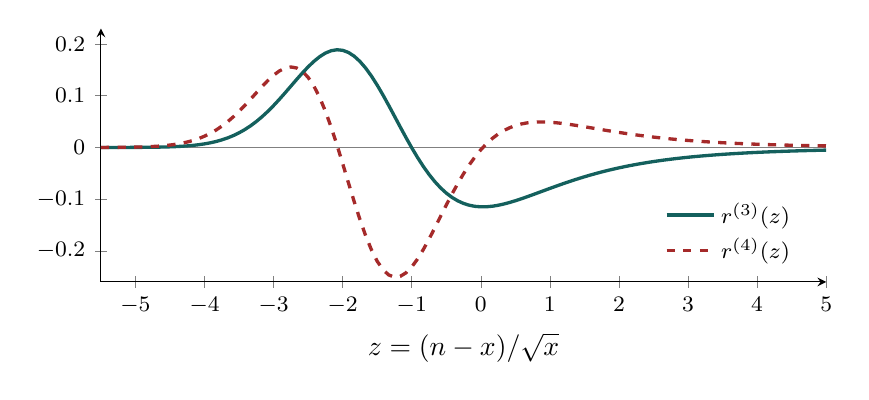
\begin{tikzpicture}
\begin{axis}[width=.89\linewidth,height=4.8cm,xmin=-5.5,xmax=5,ymin=-.26,ymax=.23,
axis lines=left, tick label style={font=\footnotesize},xlabel={$z=(n-x)/\sqrt{x}$},
ytick={-.2,-.1,0,.1,.2},xtick={-5,-4,-3,-2,-1,0,1,2,3,4,5},
legend pos=south east,legend style={draw=none,font=\footnotesize,cells={anchor=west}}]
\addplot[thin,gray,forget plot] coordinates {(-5.5,0)(5,0)};
\addplot[very thick,accent,solid] coordinates {
(-5.5000,0.000016) (-5.4167,0.000024) (-5.3333,0.000036) (-5.2500,0.000053) (-5.1667,0.000078) (-5.0833,0.000113) (-5.0000,0.000164) (-4.9167,0.000234) (-4.8333,0.000332) (-4.7500,0.000467) (-4.6667,0.000653) (-4.5833,0.000904) (-4.5000,0.001241) (-4.4167,0.001690) (-4.3333,0.002282) (-4.2500,0.003055) (-4.1667,0.004055) (-4.0833,0.005337) (-4.0000,0.006961) (-3.9167,0.009000) (-3.8333,0.011531) (-3.7500,0.014640) (-3.6667,0.018416) (-3.5833,0.022947) (-3.5000,0.028322) (-3.4167,0.034616) (-3.3333,0.041892) (-3.2500,0.050188) (-3.1667,0.059509) (-3.0833,0.069822) (-3.0000,0.081046) (-2.9167,0.093046) (-2.8333,0.105626) (-2.7500,0.118533) (-2.6667,0.131453) (-2.5833,0.144023) (-2.5000,0.155838) (-2.4167,0.166471) (-2.3333,0.175489) (-2.2500,0.182476) (-2.1667,0.187058) (-2.0833,0.188926) (-2.0000,0.187855) (-1.9167,0.183721) (-1.8333,0.176511) (-1.7500,0.166329) (-1.6667,0.153385) (-1.5833,0.137993) (-1.5000,0.120545) (-1.4167,0.101498) (-1.3333,0.081344) (-1.2500,0.060587) (-1.1667,0.039720) (-1.0833,0.019204) (-1.0000,-0.000548) (-0.9167,-0.019184) (-0.8333,-0.036422) (-0.7500,-0.052049) (-0.6667,-0.065924) (-0.5833,-0.077969) (-0.5000,-0.088168) (-0.4167,-0.096552) (-0.3333,-0.103196) (-0.2500,-0.108205) (-0.1667,-0.111707) (-0.0833,-0.113845) (0.0000,-0.114771) (0.0833,-0.114636) (0.1667,-0.113590) (0.2500,-0.111776) (0.3333,-0.109329) (0.4167,-0.106370) (0.5000,-0.103012) (0.5833,-0.099352) (0.6667,-0.095478) (0.7500,-0.091465) (0.8333,-0.087375) (0.9167,-0.083264) (1.0000,-0.079175) (1.0833,-0.075145) (1.1667,-0.071202) (1.2500,-0.067370) (1.3333,-0.063665) (1.4167,-0.060100) (1.5000,-0.056683) (1.5833,-0.053420) (1.6667,-0.050312) (1.7500,-0.047361) (1.8333,-0.044564) (1.9167,-0.041919) (2.0000,-0.039422) (2.0833,-0.037068) (2.1667,-0.034851) (2.2500,-0.032766) (2.3333,-0.030807) (2.4167,-0.028967) (2.5000,-0.027241) (2.5833,-0.025622) (2.6667,-0.024104) (2.7500,-0.022681) (2.8333,-0.021348) (2.9167,-0.020100) (3.0000,-0.018931) (3.0833,-0.017835) (3.1667,-0.016809) (3.2500,-0.015848) (3.3333,-0.014948) (3.4167,-0.014105) (3.5000,-0.013315) (3.5833,-0.012574) (3.6667,-0.011879) (3.7500,-0.011228) (3.8333,-0.010618) (3.9167,-0.010044) (4.0000,-0.009507) (4.0833,-0.009002) (4.1667,-0.008527) (4.2500,-0.008082) (4.3333,-0.007663) (4.4167,-0.007269) (4.5000,-0.006898) (4.5833,-0.006550) (4.6667,-0.006222) (4.7500,-0.005912) (4.8333,-0.005621) (4.9167,-0.005347) (5.0000,-0.005088)};
\addlegendentry{$r^{(3)} (z)$}
\addplot[very thick,Brown,dashed] coordinates {
(-5.5000,0.000079) (-5.4167,0.000117) (-5.3333,0.000170) (-5.2500,0.000247) (-5.1667,0.000354) (-5.0833,0.000504) (-5.0000,0.000711) (-4.9167,0.000994) (-4.8333,0.001378) (-4.7500,0.001895) (-4.6667,0.002581) (-4.5833,0.003484) (-4.5000,0.004661) (-4.4167,0.006176) (-4.3333,0.008108) (-4.2500,0.010543) (-4.1667,0.013574) (-4.0833,0.017302) (-4.0000,0.021830) (-3.9167,0.027256) (-3.8333,0.033666) (-3.7500,0.041125) (-3.6667,0.049665) (-3.5833,0.059272) (-3.5000,0.069873) (-3.4167,0.081319) (-3.3333,0.093379) (-3.2500,0.105722) (-3.1667,0.117918) (-3.0833,0.129440) (-3.0000,0.139672) (-2.9167,0.147929) (-2.8333,0.153491) (-2.7500,0.155641) (-2.6667,0.153713) (-2.5833,0.147152) (-2.5000,0.135561) (-2.4167,0.118761) (-2.3333,0.096825) (-2.2500,0.070106) (-2.1667,0.039242) (-2.0833,0.005134) (-2.0000,-0.031092) (-1.9167,-0.068149) (-1.8333,-0.104668) (-1.7500,-0.139286) (-1.6667,-0.170730) (-1.5833,-0.197899) (-1.5000,-0.219923) (-1.4167,-0.236214) (-1.3333,-0.246476) (-1.2500,-0.250708) (-1.1667,-0.249176) (-1.0833,-0.242373) (-1.0000,-0.230966) (-0.9167,-0.215741) (-0.8333,-0.197543) (-0.7500,-0.177226) (-0.6667,-0.155611) (-0.5833,-0.133447) (-0.5000,-0.111389) (-0.4167,-0.089988) (-0.3333,-0.069679) (-0.2500,-0.050791) (-0.1667,-0.033545) (-0.0833,-0.018076) (0.0000,-0.004438) (0.0833,0.007379) (0.1667,0.017434) (0.2500,0.025824) (0.3333,0.032670) (0.4167,0.038111) (0.5000,0.042293) (0.5833,0.045363) (0.6667,0.047465) (0.7500,0.048735) (0.8333,0.049302) (0.9167,0.049282) (1.0000,0.048779) (1.0833,0.047887) (1.1667,0.046688) (1.2500,0.045252) (1.3333,0.043641) (1.4167,0.041905) (1.5000,0.040089) (1.5833,0.038228) (1.6667,0.036352) (1.7500,0.034484) (1.8333,0.032643) (1.9167,0.030844) (2.0000,0.029099) (2.0833,0.027415) (2.1667,0.025799) (2.2500,0.024253) (2.3333,0.022781) (2.4167,0.021384) (2.5000,0.020060) (2.5833,0.018810) (2.6667,0.017630) (2.7500,0.016520) (2.8333,0.015477) (2.9167,0.014497) (3.0000,0.013579) (3.0833,0.012718) (3.1667,0.011912) (3.2500,0.011158) (3.3333,0.010454) (3.4167,0.009795) (3.5000,0.009179) (3.5833,0.008604) (3.6667,0.008067) (3.7500,0.007566) (3.8333,0.007098) (3.9167,0.006661) (4.0000,0.006253) (4.0833,0.005872) (4.1667,0.005516) (4.2500,0.005183) (4.3333,0.004873) (4.4167,0.004583) (4.5000,0.004312) (4.5833,0.004058) (4.6667,0.003821) (4.7500,0.003600) (4.8333,0.003392) (4.9167,0.003198) (5.0000,0.003017)};
\addlegendentry{$r^{(4)} (z)$}
\end{axis}
\end{tikzpicture}
\caption{The third and fourth derivatives of the limiting inverse Mills ratio. Opposite signs at separated sample points persist for the scaled remainder differences. The curves illustrate the limit in Lemma~\ref{lem:window}.}
\end{figure}

\begin{lemma}\label{lem:logwindow}
For $a>-1$ extend the normalized remainder by $\phi_a(x)=(a+1)I_x(a)$ and put $\theta_a(x)=x^{-1}\log\phi_a(x)$. For each fixed $k\ge3$,
\[
 x^{1+k/2}\,\Delta^k\theta_{x+z\sqrt x}(x)\longrightarrow
             -r^{(k-1)}(z)
\]
locally uniformly on the real line. In particular, at every sufficiently large $x$ some integer $n\ge0$ satisfies $\Delta^4\theta_n(x)<0$.
\end{lemma}
\begin{proof}
At $a=x+z\sqrt x$,
\[
 \log\phi_a(x)=\tfrac12\log x+
 \log(1+z/\sqrt x+1/x)+\log J_x(z).
\]
On neighborhoods of compact real intervals the logarithms may be chosen real on the real axis. After subtracting the constant, this expression and all fixed derivatives converge to $\log J$. Integration by parts in the defining integral gives $(\log J)'=z-r(z)$. Use the difference integral from Lemma~\ref{lem:window} and then Lemma~\ref{lem:rolle} with $k-1=3$, choosing a point where $r'''>0$ and rounding $n$ as above.
\end{proof}

\begin{corollary}
For each $k\ge4$ and all sufficiently large integers $n$, the function $x\mapsto\Delta^k\theta_n(x)$ has at least $k-3$ sign-changing zeros in $|x-n|<C'_k\sqrt n$ for some constant $C'_k$. For all sufficiently large $x$ the same lower bound holds for sign changes as the integer $n$ passes through this window, with $\sqrt{x}$ in place of $\sqrt{n}$.
\end{corollary}
\begin{proof}
Apply Lemma~\ref{lem:rolle} to $r^{(k-1)}$ and use Lemma~\ref{lem:logwindow} at the same inverse and rounded arguments as in Theorem~\ref{thm:roots}.
\end{proof}

\begin{corollary}[Sitnik's Problem 8]\label{cor:order8}
For $k\ge3$, the strict inequality $(-1)^k\Delta^k\theta_n(x)>0$ holds for all $n\ge0$ and all $x>0$ exactly when $k=3$. In the original remainder variables, at that order it is
\[
 R_n(x)R_{n+2}(x)^3>
 \frac{(n+2)(n+4)}{(n+3)^2}\,R_{n+1}(x)^3R_{n+3}(x).
\]
The factor is best possible at each $n$.
\end{corollary}
\begin{proof}
Theorem~\ref{thm:gautschi} proves the affirmative case. Inserting the defining factorials into $\phi_n\phi_{n+2}^3>\phi_{n+1}^3\phi_{n+3}$ gives precisely the displayed inequality in Problem~8. The first nonzero Taylor term of each $R_j$ gives equality in the limit of the ratio as $x\downarrow0$. For each $k\ge4$, Lemmas~\ref{lem:logwindow} and~\ref{lem:rolle} give both signs at a common sufficiently large $x$, since $r^{(k-1)}$ takes both signs. This also excludes non-strict universal inequalities at those orders.
\end{proof}

\section{A counterexample to Brezinski's 1983 suggestion}
\label{sec:rigidity}

For $x>0$ write
\[
 \phi_n(x)=\frac{(n+1)!}{x^{n+1}}R_n(x),
 \qquad \theta_n(x)=\frac{\log\phi_n(x)}x \qquad(n\ge0).
\]
A sequence $(u_n)_{n\ge0}$ is totally monotone when
$(-1)^j\Delta^j u_n\ge0$ for all $j,n\ge0$. Brezinski
\cite[p.~88]{brezinski} suggested on numerical grounds that
$(\theta_n(x))_{n\ge N}$ was totally monotone for positive $x$
at the cutoff given there. At $x=63/2$ the displayed cutoff is
$N=61$. Gautschi \cite[p.~48]{gautschi} had already reported
a negative fourth difference at $n=18$ for this same $x$.
The location of that earlier example makes the distinction between
a full sequence and one of its tails essential.

\begin{lemma}[Logarithmic moments on an arithmetic progression]
\label{lem:rigidity}
Let $\eta$ be a nonzero finite positive Borel measure on $[0,1]$
with $\eta(\{0\})=0$, and put $M_n=\int t^n\,d\eta(t)$.
Fix integers $N\ge0$ and $h\ge1$. Then
$(\log M_{N+hn})_{n\ge0}$ is totally monotone if and only if
$(\log M_n)_{n\ge0}$ is totally monotone.
\end{lemma}

\begin{proof}
By the Hausdorff moment theorem \cite{hausdorff}, total monotonicity
of a real sequence is equivalent to its representation as the moments
of a finite positive measure on $[0,1]$. If $\log M_n$ has such
a measure $\mu$, then $\log M_{N+hn}$ has representing measure
$(t\mapsto t^h)_*(t^N\mu)$.

Conversely, let $\tau$ represent $\log M_{N+hn}$. Write $*$ for
multiplicative convolution, the pushforward of a product measure
by multiplication of the coordinates. Define
\[
 E(\tau)=\delta_1+\sum_{j\ge1}\frac{\tau^{*j}}{j!}.
\]
This positive measure has finite mass $\exp(\tau([0,1]))$.
Its $n$th moment is $\exp(\int t^n\,d\tau)=M_{N+hn}$.
Uniqueness of measures with prescribed Hausdorff moments gives
\[
 E(\tau)=(t\mapsto t^h)_*(t^N\eta).
\]
The homeomorphism $s\mapsto s^{1/h}$ respects multiplication. Pushing
both sides forward by this map gives $E(\sigma)=t^N\eta$ with
$\sigma=(s\mapsto s^{1/h})_*\tau$. In particular
$\sigma\le t^N\eta$. Thus $\sigma(\{0\})=0$ and
$d\mu(t)=t^{-N}d\sigma(t)$ on $(0,1]$ defines a finite measure with
$\mu\le\eta$. Set $\mu(\{0\})=0$.
For $j\ge1$, multiplication of the variables gives
$t^{-N}\sigma^{*j}=\mu^{*j}$ on $(0,1]$. The unit mass $\delta_1$
is invariant under this weighting. Summing the positive measures yields
$E(\mu)=\eta$ on $(0,1]$, and both sides assign zero mass to $0$.
Their moments now give $\log M_n=\int t^n\,d\mu$ for every $n\ge0$.
\end{proof}

The exponential remainder fits the lemma with a positive measure
given explicitly by integration by parts in Taylor's integral formula,
\[
 \phi_n(x)=(n+1)\int_0^1 t^n e^{x(1-t)}\,dt
 =1+x\int_0^1 t^{n+1}e^{x(1-t)}\,dt,\qquad
 d\eta_x(t)=d\delta_1(t)+xt e^{x(1-t)}\,dt.
\]
Thus for each positive $x$, total monotonicity of any one progression
of $\theta_n(x)$ is equivalent to total monotonicity of the entire
sequence. In probabilistic terms the exponential of the measure is
the unnormalized compound Poisson measure, and the weight $t^N$
is an exponential tilt in the coordinate $-\log t$.

\begin{theorem}\label{thm:brezinski}
At $x=63/2$ the sequence $n\mapsto\theta_{N+hn}(x)$ fails total
monotonicity for every $N\ge0$ and every integer $h\ge1$.
In particular, at Brezinski's cutoff itself,
\[
  \Delta^{18}\theta_{61}(63/2)<0 .
\]
The same failure of total monotonicity on every progression holds
for every sufficiently large positive $x$.
\end{theorem}

\begin{proof}
We certify the displayed sign at $x=63/2$. For each
$n=61,\ldots,79$, define $T_0=1$,
$T_j=T_{j-1}x/(n+1+j)$, and $S=\sum_{j=0}^{90}T_j$. Positivity
and decreasing successive term ratios give
\[
 S<\phi_n(x)<
 S+\frac{T_{90}x}{n+92}\frac{1}{1-x/(n+93)} .
\]
For $H>1$ put $w=(H-1)/(H+1)$. The sum
$P(w)=2\sum_{i=0}^{42}w^{2i+1}/(2i+1)$ satisfies
\[
 P(w)<\log H<P(w)+\frac{2w^{87}}{87(1-w^2)} .
\]
Combining these enclosures according to the signs of the binomial
coefficients in the eighteenth difference gives
\[
 -1897143956370170171\ \le\ 
 10^{35}x\Delta^{18}\theta_{61}(x)
 \ \le\ -1897143956369735847 .
\]
Appendix~\ref{app:exact} reproduces both integers using exact rational arithmetic.
Lemma~\ref{lem:rigidity} applied to $\eta_x$ rules out total monotonicity
on every progression. For all sufficiently large $x$,
Lemma~\ref{lem:logwindow} gives a negative fourth difference of
$\theta_n(x)$ at some index, so the same argument applies.
\end{proof}


\section{A positive interval for all orders of difference}
\label{sec:smallx}

\begin{theorem}\label{thm:small}
For $0<x\le 1/10$, every $n,k\ge0$ satisfies
$(-1)^k\Delta^k\theta_n(x)>0$.
\end{theorem}

\begin{proof}
Fix $x$ in this interval. Integrating by parts, then expanding $e^{-xu}$,
gives, for real $s>0$,
\[
 F(s)=s\int_0^1 u^{s-1}e^{x(1-u)}\,du
     =1+\sum_{j\ge1}\frac{r_j}{s+j},\qquad
 r_j=xe^x\frac{(-x)^{j-1}}{(j-1)!}.
\]
Taylor's integral remainder gives $F(n+1)=\phi_n(x)$. Truncate the sum
at an even integer $m\ge2$ and call the result $F_m$. Since
$\sum_j |r_j|=xe^{2x}<1/8$, the intervals $|s+j|\le2|r_j|$ are
disjoint. On the $j$th interval the sum
$B_j(s)=\sum_{\ell\le m,\,\ell\ne j}r_\ell/(s+\ell)$ has modulus
less than $1/6$, since each denominator has modulus at least $3/4$.
The function $(s+j)F_m(s)=(s+j)(1+B_j(s))+r_j$ takes opposite
signs at the endpoints. Thus each interval contains a zero $-a_j$
of $F_m$, distinct from its pole. These $m$ zeros account for the
entire degree-$m$ numerator. Consequently
\[
 F_m(s)=\prod_{j=1}^m\frac{s+a_j}{s+j},\qquad
 a_j-j=\frac{r_j}{1+B_j(-a_j)},\qquad
 \frac67|r_j|\le |a_j-j|\le\frac65|r_j|.
\]

For odd $j<m$, both $a_j$ and $a_{j+1}$ lie in $[j,j+1]$ and
\[
 a_j+a_{j+1}-(2j+1)
 \ \ge\ \bigl(6/7-3/25\bigr)|r_j|>0,
\]
since $|r_{j+1}|/|r_j|=x/j\le1/10$. For $t>0$, bound
$u\mapsto e^{-ut}$ above by its chord on $[j,j+1]$ to get
\[
 e^{-jt}+e^{-(j+1)t}-e^{-a_jt}-e^{-a_{j+1}t}
 \ge (a_j+a_{j+1}-2j-1)(e^{-jt}-e^{-(j+1)t}).
\]
Writing $K_m(t)=\sum_{j=1}^m(e^{-jt}-e^{-a_jt})$, all pairs
therefore contribute positively, and the first pair gives
$K_m(t)\ge c_x(e^{-t}-e^{-2t})$ with
$c_x=(6/7-3/25)xe^x>0$, independently of $m$.
The integral formula for the logarithm of each linear factor yields
\[
 (-1)^k\Delta^k\log F_m(n+1)
 =\int_0^\infty e^{-(n+1)t}(1-e^{-t})^k K_m(t)\,\frac{dt}{t}.
\]
Replacing $K_m$ by its uniform lower bound gives a strictly positive
quantity independent of $m$. Taking $m\to\infty$ through even integers
on the left and dividing by $x$ proves the claim.
\end{proof}

\section{Transfer to the maximum of a Poisson sample}
Let $P$ have the Poisson law with mean $x>0$, independently of unit exponential variables $E_1,E_2,\ldots$. Put $Y_x=\max_{1\le j\le P}E_j$, with value zero when $P=0$. The parameter regions in Theorems~\ref{thm:brezinski} and~\ref{thm:small} yield statements about sums of independent random variables.

\begin{corollary}\label{cor:poissonmax}
The law of $Y_x$ is additively infinitely divisible if and only if $(\theta_n(x))_{n\ge0}$ is totally monotone. In particular it is infinitely divisible for $0<x\le1/10$. It fails additive infinite divisibility at $x=63/2$ and for every sufficiently large $x$.
\end{corollary}
\begin{proof}
Conditioning on $P$ gives $\Pr(Y_x\le y)=\exp(-xe^{-y})$ for $y\ge0$. Thus $T=e^{-Y_x}$ has law $\rho=e^{-x}\delta_1+xe^{-xt}\,dt$ on $(0,1]$. For the measure in Section~\ref{sec:rigidity} we have $\eta_x=e^x t\rho$. In particular,
\[
 e^x\mathbb E T^{n+1}=\phi_n(x).
\]
An infinitely divisible nonnegative law with an atom at zero is compound Poisson. Indeed, by the L\'evy--Khintchine representation on the positive half-line \cite{sato}, its Laplace transform has negative logarithm
$d s+\int_{(0,\infty)}(1-e^{-sy})\,\Pi(dy)$.
Here the transform tends to $e^{-x}$ as $s\to\infty$, so $d=0$ and $\Pi((0,\infty))=x$. Consequently
$\log\phi_n(x)=\int e^{-(n+1)y}\,\Pi(dy)$ has a positive Hausdorff representation.

Conversely, if $(\theta_n)$ is totally monotone, let $\mu$ represent $(\log\phi_n)$. The moment calculation in Lemma~\ref{lem:rigidity} gives $E(\mu)=\eta_x$ and $\mu\le\eta_x$. Hence $d\nu=t^{-1}d\mu$ is finite since $\int t^{-1}d\eta_x=e^x$. Weighting the convolution exponential as in the lemma gives $E(\nu)=e^x\rho$. Its total mass gives $\nu((0,1])=x$, and its mass at $1$ gives $\nu(\{1\})=0$. Passing to $-\log t$ converts multiplicative convolution into addition. The law of $Y_x$ is therefore compound Poisson with jump measure $(-\log)_*\nu$ (the pushforward under $t\mapsto-\log t$).
\end{proof}

\section{What the proofs establish}
Gautschi's third-order inequality holds on both half-axes. In Sitnik's Problem~8 this is the last order with a universal alternating sign. In Problem~11 the order classification is unconditional on the original domain. Theorem~\ref{thm:matching} gives oscillations uniformly for $k\le x/4-1$. Theorem~\ref{thm:roots} locates oscillations in a square-root window for each fixed $k$. These are distinct quantifiers. Neither estimate identifies the exact number of zeros.

For Brezinski's question, a negative value at the proposed cutoff refutes the universal statement. Theorem~\ref{thm:brezinski} further excludes every later cutoff, including on arithmetic progressions, for the specified $x$. Theorem~\ref{thm:small} gives a nonempty positive interval where every sign is strict. Determining the full set of admissible positive arguments remains outside the results of this manuscript.

\paragraph{Literature and priority.}
The primary statements appear in \cite{gautschi,sitnik,brezinski}. Low orders and earlier finite failures are credited in Section~1 and Section~\ref{sec:rigidity}. Searches for differences of exponential remainder ratios, Poisson upper-tail ratios, incomplete-gamma shape differences, Gautschi mean-value points, and total monotonicity on tails located the sources listed below. Qi's survey \cite{qi} also treats the normalized remainders and their monotonicity in the argument. The corpus check used revision \texttt{c2ac34ea4622} \cite{vmrc}. We did not locate an earlier proof of Gautschi's positive-argument third-order claim, either full order classification, or the conclusion about every tail in Brezinski's setting. This is a bounded literature finding. An independent priority assessment remains open.

The discrete Rolle argument, graph matching recurrence, Gaussian transition, Hausdorff moment theorem and exponential tilt all have classical foundations. The target-specific steps include the representation by a clipped distribution with a positive third central moment, the positivity transfer from Poisson masses to their tail ratios, the passage from derivatives of a common limiting integral to sign-changing zeros, and the application of moment uniqueness to the proposed cutoffs. Bennett \cite{bennett} gives earlier results on exponentiation and total monotonicity. The clipped precursor constructed in the proof of Theorem~\ref{thm:gautschi} is essential to the skewness argument. The clipping inequality itself is covered by van Zwet \cite{vanzwet}.

\appendix
\section{Executable certificate for the eighteenth difference}\label{app:exact}
\noindent The following Python 3 certificate uses only the standard library.
\begin{Verbatim}[fontsize=\small]
from fractions import Fraction as F
from math import ceil, comb, floor

x, B = F(63, 2), 10**35
lower, upper = [], []
for n in range(61, 80):
    term = total = F(1)
    for j in range(1, 91):
        term *= x / (n + 1 + j)
        total += term
    tail = term * x / (n + 92) / (1 - x / (n + 93))
    a = F(floor(B * total), B)
    b = F(ceil(B * (total + tail)), B)
    u, v = (a - 1)/(a + 1), (b - 1)/(b + 1)

    def partial(w):
        return 2 * sum(w**(2*i+1)/(2*i+1) for i in range(43))

    lower.append(floor(B * partial(u)))
    upper.append(ceil(B * (partial(v) + 2*v**87/(87*(1-v*v)))))

lo = sum(comb(18, i) * (lower[i] if i % 2 == 0 else -upper[i])
         for i in range(19))
hi = sum(comb(18, i) * (upper[i] if i % 2 == 0 else -lower[i])
         for i in range(19))
assert (lo, hi) == (-1897143956370170171, -1897143956369735847)
\end{Verbatim}

\begin{thebibliography}{99}\small
\bibitem{bennett} G. Bennett, Lower bounds for matrices II, \emph{Canad. J. Math.} \textbf{44} (1992), 54--74. \href{https://doi.org/10.4153/CJM-1992-003-9}{doi:10.4153/CJM-1992-003-9}.
\bibitem{brezinski} C. Brezinski, On the successive remainders of the exponential series, \emph{Elem. Math.} \textbf{38} (1983), 86--89. See the final sentence on p.~88. \href{https://doi.org/10.5169/seals-37189}{Digitized original}.
\bibitem{dlmf} NIST Digital Library of Mathematical Functions, \href{https://dlmf.nist.gov/8.12}{\S8.12, Uniform Asymptotic Expansions for Large Parameter}.
\bibitem{gautschi} W. Gautschi, A note on the successive remainders of the exponential series, \emph{Elem. Math.} \textbf{37} (1982), 46--49. \href{https://gdz.sub.uni-goettingen.de/download/pdf/PPN378850199_0037/PPN378850199_0037.pdf}{Digitized original, pp.~48--49}.
\bibitem{goldstein} L. Goldstein and G. Reinert, Distributional transformations, orthogonal polynomials, and Stein characterizations, \emph{J. Theoret. Probab.} \textbf{18} (2005), 237--260. \href{https://doi.org/10.1007/s10959-004-2602-6}{doi:10.1007/s10959-004-2602-6}.
\bibitem{hausdorff} F. Hausdorff, Summationsmethoden und Momentfolgen I, II, \emph{Math. Z.} \textbf{9} (1921), 74--109 and 280--299.
\bibitem{kw} M. Kwa\'snicki and J. Wszo\l a, Bell-shaped sequences, \emph{Studia Math.} \textbf{271} (2023), 151--185. \href{https://doi.org/10.4064/sm220923-2-2}{doi:10.4064/sm220923-2-2}.
\bibitem{mehrez} K. Mehrez and S. M. Sitnik, Proofs of some conjectures on monotonicity of ratios of Kummer, Gauss and generalized hypergeometric functions, \emph{Analysis} \textbf{36} (2016). \href{https://doi.org/10.1515/anly-2015-0029}{doi:10.1515/anly-2015-0029}. \href{https://arxiv.org/abs/1410.6120}{arXiv:1410.6120}.
\bibitem{pinelis} I. Pinelis, Exact bounds on the inverse Mills ratio and its derivatives, \emph{Complex Anal. Oper. Theory} \textbf{13} (2019), 1643--1651. \href{https://doi.org/10.1007/s11785-018-0765-x}{doi:10.1007/s11785-018-0765-x}.
\bibitem{qi} F. Qi, \emph{Theory of Normalized Remainders in Taylor Series Expansions}, 2025, revised 2026. \href{https://arxiv.org/abs/2512.15797v4}{arXiv:2512.15797v4}, Chapter~12.
\bibitem{sato} K. Sato, \emph{L\'evy Processes and Infinitely Divisible Distributions}, Cambridge University Press, 1999, Chapter~6.
\bibitem{sitnik} S. M. Sitnik, \emph{Inequalities for the exponential remainder of the Taylor series}, Vladivostok preprint, 1993, with later notes. Problems~8 and~11, pp.~23--24 and 27--28 of \href{https://arxiv.org/pdf/1608.08784v2}{arXiv:1608.08784v2}.
\bibitem{tru} TruReTuring, \href{https://www.trureturing.org/research/sitnik-1993-exponential-remainder-differences/}{A negative third difference of exponential remainder ratios}, public problem dossier, consulted 21 November 2026. See the recorded formal witness, small-argument expansion, and remaining even-order question.
\bibitem{vanzwet} W. R. van Zwet, \emph{Convex Transformations of Random Variables}, Mathematical Centre Tracts 7, Amsterdam, 1964. \href{https://ir.cwi.nl/pub/13087/13087D.pdf}{Theorem~2.2.1}.
\bibitem{vmrc} \emph{Verifiable Mathematical Reasoning Corpus}, \href{https://github.com/QEEDDD/Verifiable-Mathematical-Reasoning-Corpus/tree/c2ac34ea4622778187173f41bb1996deee8081b7}{revision c2ac34ea4622}. Items 123, \emph{Neighborhoods, Kernels and Fractional Zeros} (section on derivative signs of exponential remainders), and 204, \emph{Differences of Motzkin numbers at dyadic indices and at increasing orders}.
\end{thebibliography}
\end{document}
